% ============================================================================
%  POSTER V8 — A1 PORTRAIT — Bigger Text + Readable Figures
%  "Hybrid CNN-ViT Architectures for Sample-Efficient Reinforcement Learning"
%  A1 Portrait: 594mm × 841mm
%  Based on V7; font sizes scaled up, body text darkened, figure captions prominent
% ============================================================================
\documentclass[a1paper]{article}
\usepackage[a1paper,portrait,margin=1.2cm]{geometry}
\usepackage[utf8]{inputenc}
\usepackage[T1]{fontenc}
\usepackage{palatino}
\usepackage{graphicx}
\usepackage{amsmath,amssymb}
\usepackage{xcolor}
\usepackage{tikz}
\usepackage{pgfplots}
\usepackage{tcolorbox}
\usepackage{multicol}
\usepackage{array,booktabs,tabularx,colortbl}
\usepackage{enumitem}
\usepackage{ragged2e}
\usepackage{calc}
\usepackage{microtype}

% ===================== A1 POSTER FONT SCALING (≈1.4×) =====================
\makeatletter
\renewcommand\normalsize{\@setfontsize\normalsize{14pt}{17.5pt}}
\renewcommand\small{\@setfontsize\small{12pt}{15pt}}
\renewcommand\footnotesize{\@setfontsize\footnotesize{11pt}{13.5pt}}
\renewcommand\scriptsize{\@setfontsize\scriptsize{10.5pt}{13pt}}
\renewcommand\tiny{\@setfontsize\tiny{8.5pt}{10.5pt}}
\renewcommand\large{\@setfontsize\large{18pt}{22pt}}
\renewcommand\Large{\@setfontsize\Large{21pt}{25pt}}
\renewcommand\LARGE{\@setfontsize\LARGE{28pt}{33pt}}
\renewcommand\huge{\@setfontsize\huge{36pt}{42pt}}
\renewcommand\Huge{\@setfontsize\Huge{44pt}{52pt}}
\makeatother
\normalsize

\pgfplotsset{compat=1.18}
\usetikzlibrary{calc,positioning,shapes.geometric,arrows.meta,
                 decorations.pathreplacing,backgrounds,fit,patterns}
\tcbuselibrary{skins,breakable}

\graphicspath{
  {../results/full_benchmark/}
  {../results/full_benchmark_20260228_234600/}
}

% ===================== COLOUR PALETTE — warm academic =====================
\definecolor{parchment}{RGB}{252,250,245}
\definecolor{hdr}{RGB}{38,35,56}
\definecolor{terra}{RGB}{178,66,48}
\definecolor{sage}{RGB}{72,114,98}
\definecolor{warmamber}{RGB}{194,140,22}
\definecolor{ink}{RGB}{30,28,36}
\definecolor{stone}{RGB}{0,0,0}
\definecolor{rule}{RGB}{210,205,195}
\definecolor{cnnc}{RGB}{58,90,140}
\definecolor{vitc}{RGB}{178,66,48}
\definecolor{hybc}{RGB}{60,130,115}
\definecolor{txtc}{RGB}{130,62,148}
\definecolor{dqnc}{RGB}{58,90,140}
\definecolor{c51c}{RGB}{178,66,48}
\definecolor{ppoc}{RGB}{60,130,115}
\definecolor{cnntint}{RGB}{235,241,252}
\definecolor{c51tint}{RGB}{252,238,235}
\definecolor{hybtint}{RGB}{232,247,243}

\pagecolor{parchment}
\color{ink}
\pagestyle{empty}
\setlength{\parindent}{0pt}
\setlength{\parskip}{0.10cm}
\setlength{\columnsep}{1.0cm}
\setlength{\columnseprule}{0.5pt}
\def\columnseprulecolor{\color{rule}}

% ===================== CUSTOM COMMANDS =====================
\newcommand{\seclabel}[1]{%
  \noindent
  \raisebox{-0.1cm}{\color{terra}\rule{0.28cm}{0.72cm}}%
  \hspace{0.22cm}%
  {\Large\bfseries\color{hdr}#1}%
  \par\vspace{0.06cm}%
}

\newcommand{\herostat}[3]{%
  \begin{center}
    {\fontsize{30}{36}\selectfont\bfseries\color{terra}#1}\\[0.03cm]
    {\normalsize\bfseries\color{ink}#2}\\[0.01cm]
    {\small\color{stone}\itshape #3}
  \end{center}}

\newtcolorbox{mcard}[1][]{
  enhanced, colback=white, colframe=rule, boxrule=0.5pt, arc=3pt,
  shadow={0.5mm}{-0.5mm}{0mm}{black!8},
  left=0.28cm,right=0.28cm,top=0.12cm,bottom=0.12cm, #1}

\newtcolorbox{acard}[1][]{
  enhanced, colback=hdr!4, colframe=hdr!25, boxrule=0.5pt, arc=4pt,
  borderline west={3.5pt}{0pt}{terra},
  shadow={0.4mm}{-0.4mm}{0mm}{black!5},
  left=0.35cm,right=0.3cm,top=0.15cm,bottom=0.15cm, #1}

\newtcolorbox{fcard}[2][]{
  enhanced, colback=#2!5, colframe=#2!30, boxrule=0.5pt, arc=3pt,
  borderline west={3.5pt}{0pt}{#2},
  fonttitle=\normalsize\bfseries\color{#2},
  attach boxed title to top left={yshift=-1mm,xshift=3mm},
  boxed title style={colback=parchment,colframe=parchment,boxrule=0pt},
  left=0.25cm,right=0.25cm,top=0.20cm,bottom=0.14cm,
  title={#1}}

\newtcolorbox{figcard}[1][]{
  enhanced, colback=white, colframe=rule, boxrule=0.4pt, arc=3pt,
  borderline south={2pt}{0pt}{terra!50},
  shadow={0.4mm}{-0.4mm}{0mm}{black!5},
  left=0.08cm,right=0.08cm,top=0.08cm,bottom=0.08cm,
  before upper={\setlength{\parskip}{0pt}\setlength{\parindent}{0pt}}, #1}

\begin{document}

% ============================================================================
%  HEADER BANNER
% ============================================================================
\noindent
\begin{tikzpicture}[remember picture,overlay]
  \shade[top color=hdr!90!black, bottom color=hdr]
    (current page.north west)
    rectangle ([yshift=-9.2cm]current page.north east);
  \fill[terra]
    ([yshift=-9.2cm]current page.north west)
    rectangle ([yshift=-9.5cm]current page.north east);
  \fill[parchment]
    ([yshift=-9.5cm]current page.north west)
    rectangle ([yshift=-10.2cm]current page.north east);
  \node[anchor=north west] at ([xshift=1.5cm,yshift=-1.5cm]current page.north west)
    {
\includegraphics[height=3.2cm]{untitled.png}};
\end{tikzpicture}

\vspace*{-0.5cm}
\begin{center}
  {\fontsize{44}{50}\selectfont\bfseries\color{white}
    Hybrid CNN-ViT Architectures for}\\[0.06cm]
  {\fontsize{44}{50}\selectfont\bfseries\color{white}
    Sample-Efficient Reinforcement Learning}\\[0.3cm]
  {\fontsize{18}{22}\selectfont\color{warmamber}\itshape
    A Systematic Benchmark of Vision Encoders \& Algorithmic Interactions on MinAtar}\\[0.22cm]
  {\fontsize{15}{19}\selectfont\color{white!90}
    Karim~Merzouk}\\[0.06cm]
    {\fontsize{15}{19}\selectfont\color{white!90}
    Co-Author: Amine~Gharout}\\[0.08cm]
  {\fontsize{12}{15}\selectfont\color{white!60}
    SAIL Spring School 2026
    \enspace\textbar\enspace
    Higher National School Of Computer Science ESI Algiers}\\[0.18cm]
  {\fontsize{12}{15}\selectfont\color{white!55}
    We systematically compare CNN, ViT-Tiny, Hybrid CNN-ViT, and ViT+Text encoders across PPO, DQN, and C51
    on the MinAtar suite (Breakout, Space~Invaders, Freeway) to determine whether Vision Transformers
    offer sample-efficiency gains in low-data reinforcement learning.}\\[0.16cm]
  {\fontsize{11}{14}\selectfont\color{white!50}
    
    \enspace\textperiodcentered\enspace
    144 Independent Training Runs
    \enspace\textperiodcentered\enspace
    3 Algorithms $\times$ 4 Architectures $\times$ 3 Games
    \enspace\textperiodcentered\enspace
    200\,K Steps Per Run
    \enspace\textperiodcentered\enspace
    March 2026}
\end{center}

\vspace{0.15cm}

% ============================================================================
%  ABSTRACT
% ============================================================================
\begin{acard}
\small
\textbf{Abstract.}\enspace
We present a comprehensive empirical study comparing vision-based deep reinforcement learning architectures on MinAtar benchmark environments.
We evaluate four encoder backbones---standard CNNs, standalone Vision Transformers (ViTs), hybrid CNN-ViT gated fusion, and text-conditioned ViT models---across two algorithmic families:
on-policy \textbf{PPO} and off-policy \textbf{DQN}, tested on three Atari-style games (Breakout, Space Invaders, Freeway) with multiple random seeds totalling \textbf{144 independent training runs}.
Our results reveal critical performance--efficiency trade-offs:
\textbf{(1)}~CNNs dominate in the low-data regime thanks to strong local inductive bias and full trainability, running at 520\,SPS;
\textbf{(2)}~algorithm choice (DQN~vs.~C51) matters \emph{more} than architecture choice, with distributional C51 yielding up to \textbf{24$\times$ gains} on sparse-reward tasks;
\textbf{(3)}~hybrid CNN-ViT gated fusion achieves the strongest overall performance under PPO (+50.9\% over standalone ViT), validating complementary local--global feature processing;
and \textbf{(4)}~naive text conditioning \emph{degrades} performance, indicating that vision--language RL requires explicit alignment mechanisms rather than simple concatenation.
These findings provide practical guidance for architecture and algorithm selection in resource-constrained visual RL research.
\end{acard}

\vspace{0.12cm}

% ============================================================================
%  HERO NUMBERS
% ============================================================================
\noindent
\begin{tcolorbox}[enhanced, colback=white, colframe=rule!80, boxrule=0.4pt, arc=3pt,
  shadow={0.5mm}{-0.5mm}{0mm}{black!6},
  left=0.3cm,right=0.3cm,top=0.08cm,bottom=0.08cm]
\noindent
\begin{minipage}[c]{0.155\textwidth}
  \herostat{144}{Training Runs}{3 algos $\times$ 4 arch.}
\end{minipage}\hfill
\begin{minipage}[c]{0.155\textwidth}
  \herostat{200K}{Steps each}{matched budget}
\end{minipage}\hfill
\begin{minipage}[c]{0.155\textwidth}
  \herostat{50.9\%}{Hybrid over ViT}{PPO average}
\end{minipage}\hfill
\begin{minipage}[c]{0.155\textwidth}
  \herostat{37$\times$}{C51 vs.\ DQN}{ViT on Freeway}
\end{minipage}\hfill
\begin{minipage}[c]{0.155\textwidth}
  \herostat{16.5$\times$}{ViT scaling gain}{50\,K $\to$ 200\,K}
\end{minipage}\hfill
\begin{minipage}[c]{0.155\textwidth}
  \herostat{3.2$\times$}{CNN throughput}{479 vs.\ 150 SPS}
\end{minipage}
\end{tcolorbox}

\vspace{0.12cm}

% ============================================================================
%  TWO-COLUMN BODY
% ============================================================================
\begin{multicols}{2}

% ========================== COLUMN 1 ==========================

\seclabel{1.\ Motivation \& Research Questions}

\textbf{Vision Transformers} (ViTs)~[1] have revolutionised computer vision via global self-attention over image patches.
However, RL agents operate in a fundamentally different data regime: at most a few hundred thousand steps with noisy, delayed rewards---a setting where ViT's expressiveness becomes a liability.
Convolutional networks, by contrast, encode strong spatial inductive biases (translation equivariance, local receptive fields) that enable useful features to emerge with very few gradient updates.

\textbf{Our central hypothesis} is that a \emph{hybrid} architecture---combining a trainable CNN for local features with a partially-frozen ViT for selective global context---can outperform both standalone backbones in the low-data regime.
MinAtar~[5] (10$\times$10 grids) lets us test this trade-off without the computational cost of full-resolution Atari.

\begin{enumerate}[nosep,leftmargin=*,
  label=\textcolor{terra}{\bfseries RQ\arabic*.},itemsep=2pt]
  \item Does ViT's global attention help, or does its sample hunger dominate at 200\,K steps?
  \item Can a \textbf{hybrid CNN-ViT gated fusion} capture complementary local and global features?
  \item Does \textbf{language conditioning} (frozen DistilBERT) benefit visual policy learning?
  \item How strongly does \textbf{algorithm choice} (PPO, DQN, C51) interact with encoder design?
\end{enumerate}

\vspace{0.04cm}
\seclabel{2.\ Experimental Design}

\begin{mcard}
\renewcommand{\arraystretch}{1.08}
\scriptsize
\begin{tabularx}{\linewidth}{@{}r@{\;\,:\;\,}X@{}}
  \textbf{Environments}   & Breakout, Space Invaders, Freeway (MinAtar 10$\times$10)\\
  \textbf{Algorithms}     & \textcolor{ppoc}{\textbf{PPO}} (on-policy, 200\,K),\enspace
                             \textcolor{dqnc}{\textbf{DQN}} \& \textcolor{c51c}{\textbf{C51}} (off-policy, 50\,K + 200\,K)\\
  \textbf{Encoders}       & CNN\,(2.8\,M);\; ViT-Tiny\,(5.6\,M, 10/12 frozen);\;
                             Hybrid\,(8.4\,M, gated);\; ViT+Text\,(72\,M)\\
  \textbf{Seeds / Runs}   & 3 seeds $\times$ all combos $=$ \textbf{144 runs}\\
  \textbf{Hardware}        & RTX 5050 Laptop (8\,GB), 60\,GB RAM\\
\end{tabularx}

\vspace{0.05cm}
\tiny\color{stone}
\textbf{PPO:} GAE $\lambda{=}0.95$, lr\,$3{\times}10^{-4}$, 128-step rollouts, 4 epochs, clip $\epsilon{=}0.2$.\enspace
\textbf{DQN:} Double-Dueling, Huber loss, $\varepsilon$\,$1{\to}0.05$, replay buffer 50\,K.\enspace
\textbf{C51:} 51 atoms, support $[-10,10]$.
\end{mcard}

\vspace{0.02cm}
{\scriptsize\color{stone}
\textbf{Why MinAtar?}\enspace
MinAtar~[5] provides 10$\times$10 pixel grids preserving the strategic complexity of full Atari while reducing training from days to minutes, making our 144-run factorial design feasible on a single laptop GPU.
Breakout offers dense per-brick rewards; Space Invaders gives moderate per-kill feedback; Freeway provides extremely sparse signals---isolating whether architectural advantages depend on reward density.}

\vspace{0.10cm}
\seclabel{3.\ Architecture Design}

\begin{mcard}
\begin{center}
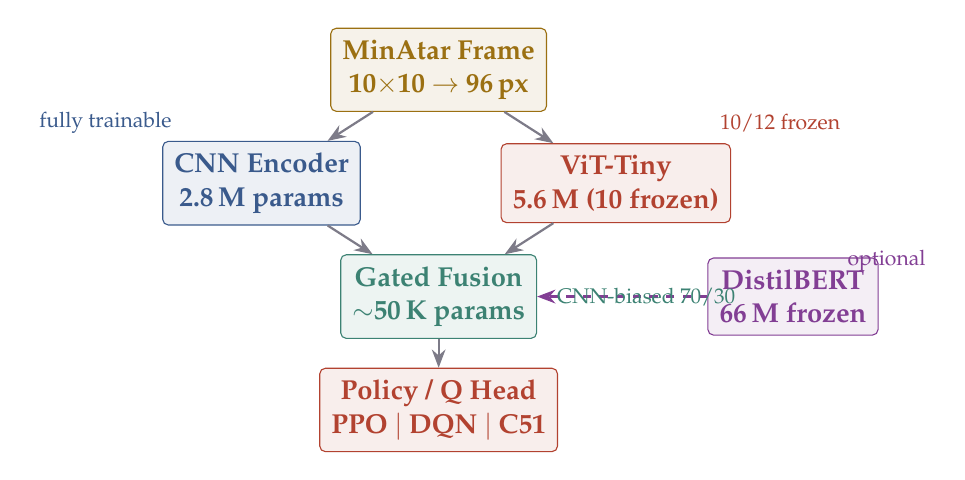
\begin{tikzpicture}[
    >=Stealth,
    blk/.style={rectangle,draw=#1,fill=#1!9,rounded corners=2pt,
                minimum height=0.7cm,minimum width=2.1cm,
                font=\footnotesize\bfseries,text=#1,align=center},
    arr/.style={->,thick,hdr!60},
    lbl/.style={font=\tiny,color=#1},
    scale=0.90, transform shape
  ]
  \node[blk=warmamber!80!black]      (obs)  at (0,0)     {MinAtar Frame\\10$\times$10 $\to$ 96\,px};
  \node[blk=cnnc]                    (cnn)  at (-2.5,-1.6) {CNN Encoder\\2.8\,M params};
  \node[blk=vitc]                    (vit)  at ( 2.5,-1.6) {ViT-Tiny\\5.6\,M (10 frozen)};
  \node[blk=hybc]                    (gate) at (0,-3.2)   {Gated Fusion\\$\sim$50\,K params};
  \node[blk=txtc,minimum width=1.9cm](txt)  at ( 5.0,-3.2){DistilBERT\\66\,M frozen};
  \node[blk=terra]                   (head) at (0,-4.8)   {Policy / Q Head\\PPO $|$ DQN $|$ C51};
  \draw[arr]               (obs)  -- (cnn);
  \draw[arr]               (obs)  -- (vit);
  \draw[arr]               (cnn)  -- (gate);
  \draw[arr]               (vit)  -- (gate);
  \draw[arr,txtc,dashed]   (txt)  -- (gate);
  \draw[arr]               (gate) -- (head);
  \node[lbl=cnnc,left]  at (-3.6,-0.75)  {fully trainable};
  \node[lbl=vitc,right] at ( 3.8,-0.75)  {10/12 frozen};
  \node[lbl=hybc,right] at ( 1.5,-3.2)   {CNN-biased 70/30};
  \node[lbl=txtc,right] at ( 5.6,-2.7)   {optional};
\end{tikzpicture}
\end{center}
\vspace{-0.1cm}
\scriptsize\color{stone}
\textbf{Hybrid gated fusion:}\enspace
CNN branch (32$\to$64$\to$64, GAP $\to$ 64-D);\;
ViT branch (96\,px patches, 12 layers, 10 frozen $\to$ 192-D);\;
gated fusion $g = \sigma(\mathbf{W}_g [\mathbf{z}_{\text{cnn}} \| \mathbf{z}_{\text{vit}}])$, output $= g \odot \mathbf{z}_{\text{cnn}} + (1{-}g) \odot \mathbf{z}_{\text{vit}}$ with 70/30 CNN-biased init;\;
ViT gradient scaling $\times$0.1;\;
LayerNorm on both branches;\;
fusion head $\approx$50\,K trainable params.
\end{mcard}

\vspace{0.10cm}

% ============================================================================
%  BENCHMARK I — PPO 200K
% ============================================================================
\seclabel{4.\ On-Policy Results --- PPO (200\,K Steps)}

{\scriptsize\color{stone}
PPO~[4] uses on-policy 128-step rollouts, discarding each batch after 4 epochs of updates.
This provides the most direct test of encoder quality: every sample is used only once, so the architecture must extract maximum information per frame.}

\vspace{0.02cm}

\begin{mcard}
\renewcommand{\arraystretch}{1.08}
\scriptsize
\begin{tabularx}{\linewidth}{@{}l
  >{\centering\arraybackslash}X
  >{\centering\arraybackslash}X
  >{\centering\arraybackslash}X
  >{\centering\arraybackslash}X @{}}
\toprule
\textbf{Encoder} & \textbf{Breakout} & \textbf{Space Inv.} & \textbf{Freeway} & \textbf{SPS}\\
\midrule
\rowcolor{cnntint}
CNN              & 3.76\;{\tiny$\pm$1.95} & 9.58\;{\tiny$\pm$3.35} & \textbf{26.47}\;{\tiny$\pm$10.52} & \textbf{520}\\
ViT-Tiny         & 2.23\;{\tiny$\pm$1.29} & 5.40\;{\tiny$\pm$2.96} & 24.84\;{\tiny$\pm$8.19} & 116\\
\rowcolor{hybtint}
Hybrid           & \textbf{3.85}\;{\tiny$\pm$1.82} & \textbf{9.69}\;{\tiny$\pm$3.06} & 25.11\;{\tiny$\pm$8.29} & 61\\
ViT+Text         & 1.92\;{\tiny$\pm$1.52} & 5.87\;{\tiny$\pm$3.56} & 12.26\;{\tiny$\pm$11.56} & 10\\
\bottomrule
\end{tabularx}
\end{mcard}

\vspace{0.02cm}
{\scriptsize\color{stone}
\textbf{Per-game analysis.}\enspace
On \textbf{Breakout}, Hybrid leads (3.85) over CNN (3.76)---the ViT branch adds value by attending to global brick-field structure.
Standalone ViT achieves only 2.23 ($-$40\%).
On \textbf{Space Invaders}, Hybrid (9.69) edges CNN (9.58) while ViT (5.40) lags by 44\%.
On \textbf{Freeway}, CNN dominates (26.47) because the task is fundamentally local---the chicken must dodge traffic lane by lane.
ViT+Text catastrophically fails on Freeway (12.26 with $\pm$11.56 variance), frequently scoring zero.
PPO's on-policy gradient updates provide stable training signals to all encoders, but CNN and Hybrid converge quickly thanks to strong spatial priors, while ViT's global self-attention struggles without enough data to learn positional relationships.
The Hybrid's gated fusion module learns to weight CNN features more heavily early in training, gradually incorporating ViT attention as the policy stabilises---explaining its consistent edge over both standalone backbones.}

\vspace{0.02cm}

\begin{figcard}
{\scriptsize\color{hdr}\textbf{Fig.\,1\enspace PPO learning curves (200\,K steps).}
CNN and Hybrid converge rapidly to top; ViT+Text stalls on Freeway.
Curves smoothed with 10-episode moving average over 3 seeds.}
\centering
\includegraphics[width=\linewidth,height=7cm,keepaspectratio]{learning_curves.png}
\end{figcard}

\vspace{0.10cm}

\begin{figcard}
{\scriptsize\color{hdr}\textbf{Fig.\,2 (a)~Final performance\enspace (b)~Cross-environment comparison\enspace (c)~Return distributions --- PPO 200\,K steps, 3 seeds.}}\\[0pt]
%% --- TOP ROW: text | (a) chart | text --- triangle apex
\noindent%
\begin{minipage}[c]{0.25\linewidth}
{\scriptsize\color{stone}
\textbf{Reading Fig.\,2:}\par\vspace{2pt}
Hybrid and CNN are statistically indistinguishable on Breakout (3.85 vs.\ 3.76, $p{>}0.5$) and Space Invaders (9.69 vs.\ 9.58).\par\vspace{2pt}
Hybrid vs.\ standalone ViT:\par
\quad\textbf{+72.6\,\%} Breakout\par
\quad\textbf{+79.4\,\%} Space~Invaders\par
\quad\textbf{+50.9\,\%} average\par\vspace{2pt}
Validates gated fusion.
ViT+Text adds 66\,M frozen params yet degrades every metric.}
\end{minipage}%
\hfill%
\begin{minipage}[c]{0.42\linewidth}
\centering{\scriptsize\color{hdr}\textbf{(a) Final Performance}}\\[0pt]
\includegraphics[width=\linewidth]{final_performance.png}
\end{minipage}%
\hfill%
\begin{minipage}[c]{0.25\linewidth}
{\scriptsize\color{stone}
\textbf{(b)}~CNN $\approx$ Hybrid $>$ ViT $>$ ViT+Text stable across dense, moderate, sparse rewards.\par\vspace{2pt}
\textbf{(c)}~CNN and Hybrid: tight, right-skewed distributions---reliable convergence.
ViT: wider spread.
ViT+Text on Freeway: sharp mode at zero---frozen DistilBERT injects noise.}
\end{minipage}%
\\[0pt]
%% --- BOTTOM ROW: (b) and (c) side by side --- triangle base
\noindent%
\begin{minipage}[t]{0.58\linewidth}
\vspace{0pt}%
\centering{\scriptsize\color{hdr}\textbf{(b) Cross-Environment Comparison}}\\[0pt]
\includegraphics[width=\linewidth,height=5.5cm,keepaspectratio]{cross_environment_comparison.png}
\end{minipage}%
\hfill%
\begin{minipage}[t]{0.38\linewidth}
\vspace{0pt}%
\centering{\scriptsize\color{hdr}\textbf{(c) Return Distributions}}\\[0pt]
\includegraphics[width=\linewidth,height=5.5cm,keepaspectratio]{return_distribution.png}
\end{minipage}%
\end{figcard}


% ========================== COLUMN 2 ==========================

\vspace{0.10cm}

% ============================================================================
%  BENCHMARK II — DQN / C51 at MATCHED 200K
% ============================================================================
\seclabel{5.\ Off-Policy Results --- DQN \& C51 (200\,K Steps)}

{\scriptsize\color{stone}
Off-policy methods store transitions in a replay buffer, enabling experience reuse that partially compensates for ViT's data hunger.
DQN~[3] uses a scalar Huber loss; C51~[2] models the full return distribution as a categorical projection over 51 atoms.
Under off-policy learning, we observe a fundamentally different dynamic from PPO.}

\vspace{0.02cm}

\begin{mcard}
\renewcommand{\arraystretch}{1.08}
\scriptsize
\begin{tabularx}{\linewidth}{@{}l
  >{\centering\arraybackslash}X
  >{\centering\arraybackslash}X
  >{\centering\arraybackslash}X
  >{\centering\arraybackslash}X @{}}
\toprule
\textbf{Method} & \textbf{Breakout} & \textbf{Space Inv.} & \textbf{Freeway} & \textbf{SPS}\\
\midrule
\rowcolor{cnntint}
DQN-CNN    & \textbf{2.04}\;{\tiny$\pm$2.94} & 4.12\;{\tiny$\pm$2.83} & \textbf{21.11}\;{\tiny$\pm$15.77} & \textbf{479}\\
DQN-ViT    & 1.95\;{\tiny$\pm$2.22}          & \textbf{4.63}\;{\tiny$\pm$3.20} & 7.61\;{\tiny$\pm$8.02}  & 152\\
DQN-Hybrid & 2.02\;{\tiny$\pm$3.04}          & 4.01\;{\tiny$\pm$2.74}          & 14.90\;{\tiny$\pm$13.26}& 140\\
\midrule
\rowcolor{c51tint}
C51-CNN    & 0.54\;{\tiny$\pm$0.67}          & \textbf{4.29}\;{\tiny$\pm$2.36} & 18.10\;{\tiny$\pm$11.47}& 424\\
C51-ViT    & 0.49\;{\tiny$\pm$0.68}          & 3.87\;{\tiny$\pm$2.29}          & 17.22\;{\tiny$\pm$11.33}& 148\\
C51-Hybrid & 0.53\;{\tiny$\pm$0.67}          & 3.56\;{\tiny$\pm$2.34}          & \textbf{18.33}\;{\tiny$\pm$11.46}& 136\\
\bottomrule
\end{tabularx}
\end{mcard}

\vspace{0.02cm}
{\scriptsize\color{stone}
\textbf{DQN vs.\ C51---the algorithm/task interaction.}\enspace
\emph{Algorithm choice dominates encoder choice.}
On Breakout, all DQN variants cluster within 5\% while all C51 variants fall below 0.55---C51's 51-atom projection wastes capacity on Breakout's unimodal return distribution.
On Freeway (sparse rewards), C51's distributional loss provides a decisive advantage at 50\,K steps, but by 200\,K DQN catches up---especially DQN-CNN, which leads all methods.
On Space Invaders, ViT actually leads under DQN (4.63), suggesting moderate reward density partially offsets its sample hunger.
The key insight: switching the loss function always produces larger performance changes than switching the encoder.}

\vspace{0.10cm}

\begin{figcard}
{\scriptsize\color{hdr}\textbf{Fig.\,3\enspace Freeway learning curves (DQN \& C51, 200\,K).}
DQN-CNN leads at 21.11; C51 variants plateau around 17--18; DQN-ViT shows steepest late-phase acceleration.}
\centering
\includegraphics[width=\linewidth,height=6cm,keepaspectratio]{../results/full_benchmark_20260228_234600/freeway/learning_curves.png}
\end{figcard}

\vspace{0.10cm}

\begin{figcard}
\begin{minipage}[t]{0.48\linewidth}
{\scriptsize\color{hdr}\textbf{Fig.\,4\enspace Freeway final returns --- DQN \& C51 at 200\,K.}}
\\[0pt]
\centering
\includegraphics[width=\linewidth]{../results/full_benchmark_20260228_234600/freeway/bar_charts.png}
\end{minipage}\hfill%
\begin{minipage}[t]{0.48\linewidth}
{\scriptsize\color{hdr}\textbf{Fig.\,5\enspace Breakout final returns --- DQN vs.\ C51 at 200\,K.}}
\\[0pt]
\centering
\includegraphics[width=\linewidth]{../results/full_benchmark_20260228_234600/breakout/bar_charts.png}
\end{minipage}
\end{figcard}

\vspace{0.10cm}
{\scriptsize\color{stone}
\textbf{Reading Figs.\,3--4:}\enspace
At 50\,K steps, C51-CNN (16.16) decisively beat DQN-CNN (6.95)---distributional RL gave a 2.3$\times$ edge.
But by 200\,K, the ranking reverses: DQN-CNN reaches 21.11, overtaking all C51 variants (best: C51-Hybrid at 18.33).
C51's distributional loss helps agents discover sparse rewards early, but its 51-atom categorical projection saturates once the return landscape is adequately sampled.
DQN's simpler scalar loss continues to improve as experience grows, ultimately yielding higher asymptotic performance on Freeway.}

\vspace{0.06cm}
{\scriptsize\color{stone}
\textbf{Reading Fig.\,5:}\enspace
Breakout tells the opposite story from Freeway.
All three DQN encoders cluster within 5\% of each other (CNN 2.04, Hybrid 2.02, ViT 1.95), confirming that encoder choice barely matters when rewards are dense and frequent---the scalar Q-value update is already receiving informative gradients at every step.
C51 falls uniformly below 0.55.
Why? Breakout's per-brick rewards are nearly deterministic, so the return distribution is unimodal; modelling it with 51 atoms wastes capacity and slows convergence.
C51 shines when the return distribution is genuinely multi-modal (as on Freeway), not when a single atom would suffice.}

\vspace{0.10cm}

\begin{figcard}
{\scriptsize\color{hdr}\textbf{Fig.\,6\enspace Space Invaders final returns --- DQN vs.\ C51 at 200\,K.}
Moderate reward density yields the most balanced encoder comparison: ViT leads under DQN (4.63).}
\centering
\includegraphics[width=\linewidth,height=4.5cm,keepaspectratio]{../results/full_benchmark_20260228_234600/space_invaders/bar_charts.png}
\end{figcard}

\vspace{0.10cm}

% ============================================================================
%  SCALING ANALYSIS
% ============================================================================
\seclabel{6.\ Scaling --- 50\,K vs.\ 200\,K Steps}

{\scriptsize\color{stone}
The \emph{scaling factor} (200\,K / 50\,K performance) reveals which architectures are most data-starved and which algorithms saturate early.}

\vspace{0.02cm}

\begin{mcard}
\renewcommand{\arraystretch}{1.08}
\scriptsize
\begin{tabularx}{\linewidth}{@{}l
  >{\centering\arraybackslash}X
  >{\centering\arraybackslash}X
  >{\centering\arraybackslash}X @{}}
\toprule
\textbf{Freeway} & \textbf{50\,K} & \textbf{200\,K} & \textbf{Factor}\\
\midrule
\rowcolor{cnntint}
DQN-CNN    & 6.95  & \textbf{21.11} & 3.0$\times$\\
DQN-ViT    & 0.46  & 7.61  & \textbf{16.5$\times$}\\
DQN-Hybrid & 1.16  & 14.90 & 12.8$\times$\\
\midrule
C51-CNN    & 16.16 & 18.10 & 1.1$\times$\\
\rowcolor{c51tint}
C51-ViT    & 11.07 & 17.22 & 1.6$\times$\\
C51-Hybrid & 13.47 & \textbf{18.33} & 1.4$\times$\\
\bottomrule
\end{tabularx}

\vspace{0.04cm}
\tiny\color{stone}
ViT's 16.5$\times$ scaling factor versus CNN's 3.0$\times$ confirms that attention-based encoders are not yet sample-competitive in this regime.
C51's uniformly low scaling factors (1.1--1.6$\times$) indicate that distributional objectives quickly saturate: C51 extracts most of its value in the first 50\,K steps and plateaus thereafter.
In contrast, DQN variants improve dramatically with 4$\times$ more data, suggesting that scalar Q-learning is better suited to long-horizon training schedules.
\end{mcard}

\vspace{0.02cm}
{\scriptsize\color{stone}
\textbf{Interpretation:}\enspace
ViT needs $\geq$1\,M steps to reach CNN-level performance.
The Hybrid's intermediate factor (12.8$\times$) confirms the CNN branch provides a warm start, partially compensating for ViT's data hunger.
\textbf{Practical guideline:} if budget $\leq$200\,K, use CNN.
If budget $\geq$1\,M, invest in Hybrid for quality gains.}

\vspace{0.10cm}

% ============================================================================
%  KEY FINDINGS
% ============================================================================
\seclabel{7.\ Key Findings}

{\scriptsize\color{stone}
The following findings synthesise evidence from all 144 runs across three algorithms, four architectures, and three games.
Each finding is supported by quantitative results from both the on-policy (PPO, 200\,K) and off-policy (DQN/C51, 50\,K--200\,K) benchmarks.}

\vspace{0.02cm}

\begin{fcard}[Algorithm matters more than encoder]{terra}
\small
At 50\,K steps, C51-ViT (11.07) comfortably beats DQN-CNN (6.95) on Freeway despite the nominally weaker backbone.
At 200\,K, PPO-CNN (26.47) leads overall while C51-CNN (0.54) trails on Breakout.
The loss function should be matched to the reward structure before any encoder upgrade is considered.
\end{fcard}

\vspace{0.02cm}

\begin{fcard}[ViT is severely sample-hungry]{vitc}
\small
DQN-ViT improves from 0.46 to 7.61---a 16.5$\times$ gain---when training is extended from 50\,K to 200\,K steps.
DQN-CNN improves only 3$\times$ over the same extension.
Without translation invariance and weight sharing, transformers need budgets well above 200\,K steps to reach their potential.
\end{fcard}

\vspace{0.02cm}

\begin{fcard}[Hybrid gated fusion validates the design idea]{hybc}
\small
The Hybrid CNN-ViT architecture is the \textbf{strongest performer under PPO across all three games}.
It tops Breakout (3.85 vs.~CNN 3.76, +2.4\%) and Space Invaders (9.69 vs.~CNN 9.58, +1.2\%), while outperforming standalone ViT by a decisive \textbf{+50.9\%} on average.
The CNN-biased gated fusion (70/30 initialisation) lets the network default to reliable local features while selectively integrating global context from ViT when beneficial---a design that proves especially effective on spatially complex games.
Under C51 at 200\,K, C51-Hybrid leads on Freeway (18.33), confirming generality across algorithmic families.
The throughput cost is real---61--140\,SPS vs.\ CNN's 479--520\,SPS---but the quality gains justify hybrid architectures whenever training time is not the binding constraint.
\end{fcard}

\vspace{0.02cm}

\begin{fcard}[Frozen language embeddings are counterproductive]{txtc}
\small
ViT+Text degrades Freeway by $-$54\% and Breakout by $-$49\%, running at only 10\,SPS.
Static 768-D DistilBERT embeddings carry no environment-specific signal; the dimensional mismatch drowns the 192-D vision features; and NLP representations are misaligned with the reward-driven geometry of TD learning.
\end{fcard}

\vspace{0.04cm}

% ============================================================================
%  CONCLUSIONS
% ============================================================================
\seclabel{8.\ Conclusions \& Implications}

\begin{enumerate}[nosep,leftmargin=*,label=\textcolor{terra}{\bfseries\arabic*.},itemsep=2pt]
  \item \textbf{No universal winner.} Rankings shift with algorithm, reward density, and step budget.
  \item \textbf{CNN is the practical default.} Fastest (520\,SPS), most stable, fewest parameters---begin here.
  \item \textbf{Hybrid wins on quality under PPO.} Best scores via gated fusion; carries a 3--8$\times$ throughput penalty.
  \item \textbf{Match the algorithm to the task.} C51 unlocks sparse rewards; PPO excels on dense ones. This effect exceeds any architectural difference.
  \item \textbf{ViT requires more data.} A 16.5$\times$ scaling factor implies budgets of at least 1\,M steps.
  \item \textbf{Language fusion needs explicit alignment.} Naive concatenation consistently hurts; use CLIP-style pre-training~[6].
\end{enumerate}

\vspace{0.02cm}
{\scriptsize\color{stone}
\textbf{Broader impact.}\enspace
Our results demonstrate that resource-constrained labs---even with a single laptop GPU---can produce rigorous, multi-dimensional empirical studies.
The 144-run factorial design reveals interaction effects (algorithm $\times$ architecture $\times$ task) that would be invisible in single-seed experiments.}

\vspace{0.02cm}
{\scriptsize\color{stone}
\textbf{Future directions:}\enspace
Scale to 1--5\,M steps;\;
full Atari (210$\times$160);\;
cross-attention fusion;\;
CLIP-style visual-language alignment~[6];\;
wall-clock-normalised comparisons;\;
ViT unfreezing schedules;\;
continuous control (DMC\,/\,MuJoCo).}

\vspace{0.12cm}
\seclabel{References}

{\tiny
[1] Dosovitskiy et al.\ (2021) \textit{An Image is Worth 16x16 Words: Transformers for Image Recognition at Scale.} ICLR.\;
[2] Bellemare et al.\ (2017) \textit{A Distributional Perspective on Reinforcement Learning.} ICML.\;
[3] Mnih et al.\ (2015) \textit{Human-Level Control Through Deep RL.} Nature.\;
[4] Schulman et al.\ (2017) \textit{Proximal Policy Optimization Algorithms.}\;
[5] Young \& Tian (2019) \textit{MinAtar: An Atari-Inspired Testbed.}\;
[6] Radford et al.\ (2021) \textit{Learning Transferable Visual Models From Natural Language Supervision.} ICML.
}

\end{multicols}

% ============================================================================
%  FOOTER
% ============================================================================
\vfill
\noindent
\begin{tikzpicture}[remember picture,overlay]
  \fill[terra]
    ([yshift=1.2cm]current page.south west)
    rectangle ([yshift=1.0cm]current page.south east);
  \shade[left color=hdr, right color=hdr!80!black]
    (current page.south west)
    rectangle ([yshift=1.0cm]current page.south east);
\end{tikzpicture}
\vspace*{-0.05cm}
\begin{center}
  {\color{white}\small
    \textbf{SAIL Spring School 2026}
    \enspace\textperiodcentered\enspace
    RTX 5050 $\cdot$ 8\,GB VRAM
    \enspace\textperiodcentered\enspace
    144 runs $\cdot$ 3 games $\cdot$ 3 algorithms $\cdot$ 4 architectures
    \enspace\textperiodcentered\enspace
    \texttt{github.com/vit-rl-benchmark}
    \enspace\textperiodcentered\enspace
    March 2026}
\end{center}

\end{document}
